\documentclass[12pt]{article}
\usepackage[margin=1in]{geometry}
\usepackage{graphicx}
\usepackage{amsmath}
\usepackage{float}
\usepackage{hyperref}
\usepackage{caption}
\usepackage{subcaption}
\usepackage{fancyhdr}
\usepackage{tocloft}

% Header and footer settings for page numbers
\pagestyle{fancy}
\fancyhf{}
\fancyfoot[C]{\thepage}

% Title info
\title{PyTorch Neural Network for Predicting Medical Appointment No-Shows}
\author{Abhishek Kumar Chaubey \\
Roll Number: 24144001 \\
IIT (BHU) Varanasi}
\date{\today}

\begin{document}

\maketitle

\tableofcontents
\newpage

\section*{Objective}
The objective of this assignment is to build a PyTorch-based binary classification model to predict whether a patient will show up for a medical appointment. The model must handle class imbalance without using oversampling, undersampling, or data augmentation techniques. The implementation is compared against a previously built pure Python neural network on the same dataset and data splits.

\section*{Dataset Description}
We use the ``Medical Appointment No-Show'' dataset, which contains information about over 100,000 patient appointments in Brazil. Key features include:

\begin{itemize}
    \item Age
    \item Gender
    \item Scholarship (welfare)
    \item Hypertension
    \item Diabetes
    \item Alcoholism
    \item SMS Received
    \item Days\_diff (gap between scheduling and appointment)
    \item ScheduledDayOfWeek and AppointmentDayOfWeek (numerical weekdays)
\end{itemize}

The target variable is binary:
\begin{itemize}
    \item 0: Patient showed up
    \item 1: Patient did not show up
\end{itemize}

This dataset is highly imbalanced: approximately 49894 samples belong to class 0, and 19934 to class 1.

\section*{Data Splitting Strategy}
To ensure a fair comparison with the previous implementation, the same data splits were used:
\begin{itemize}
    \item Training set (80\%)
    \item Test set (20\%)
\end{itemize}

This split was performed after scaling and then saved in \texttt{.npy} files so that the same split can be used for the PyTorch implementation.

\section*{Neural Network Architecture}
I experimented with several architectures during model development:

\begin{itemize}
    \item Initial: Two hidden layers with 8 and 8 neurons.
    \item Second attempt: Two hidden layers with 16 and 16 neurons.
    \item Final architecture: 
    \begin{itemize}
        \item Input Layer: 14 features
        \item Hidden Layer 1: 64 neurons, ReLU activation
        \item Hidden Layer 2: 32 neurons, ReLU activation
        \item Output Layer: 1 neuron, Sigmoid activation
    \end{itemize}
\end{itemize}

The final architecture provided smoother training and validation performance. He initialization was used for ReLU layers and Xavier initialization for the output layer. All biases were initialized to zero.

\section*{Why Only 1 Output Neuron?}
Since this is a binary classification task, I used a single output neuron with a sigmoid activation function. This outputs a probability score between 0 and 1, which can be thresholded at 0.5 to determine the predicted class.

Using \texttt{softmax} would only be necessary if I had multiple mutually exclusive output classes, which is not the case here.

\section*{Handling Class Imbalance (took gpt's help in this step)}
To handle the significant imbalance in the dataset, I used a \textbf{weighted Binary Cross-Entropy loss} where the positive class (no-show) was upweighted. The weight was calculated as:

\[
\text{Positive Class Weight} = \frac{\text{Total Samples}}{2 \times \text{Positive Samples}}
\]

This allowed the model to pay more attention to the minority class without altering the dataset distribution.

\section*{Learning Rate Experimentation}
Both implementations required tuning the learning rate separately for stable and effective training.

\subsection*{1. Pure Python Implementation}
In the pure Python model, I initially tried larger learning rates like \texttt{0.001}, but training was unstable and led to poor convergence. After several trials, a learning rate of \texttt{0.0008} was found to offer the best trade-off between convergence speed and performance stability. This value was manually selected based on validation loss behavior and F1 score trends.

\subsection*{2. PyTorch Implementation}
I initially used the same learning rate of \texttt{0.0008} in PyTorch as well. However, this caused erratic validation curves—loss decreased initially but then increased again, and the F1 score fluctuated in a zigzag pattern with high variance.

I then tried \texttt{0.00008}, which showed slightly improved stability but still wasn’t optimal. Finally, I settled on \texttt{0.00003}, which resulted in smooth and stable convergence across all training and validation metrics. This value was thus finalized for the PyTorch implementation.

\section*{Training Configuration}
\begin{itemize}
    \item Optimizer: Adam
    \item Loss: Binary Cross-Entropy with class weights
    \item Batch Size: 256
    \item Epochs: 200
    \item Learning Rate: 0.00003 (PyTorch), 0.0008 (Pure Python)
    \item Regularization: L2 weight decay (1e-4)
\end{itemize}

\section*{Evaluation Metrics}
The models were evaluated on the test set using:

\begin{itemize}
    \item Accuracy
    \item F1 Score
    \item ROC AUC
    \item Precision-Recall AUC (PR AUC)
    \item Confusion Matrix
\end{itemize}

\section*{Results on Test Set}

\begin{itemize}
    \item \textbf{Accuracy:} 0.6822 (Pure Python Implementation)
    \item \textbf{F1 Score:} 0.2627 (Pure Python Implementation)
    \item \textbf{ROC AUC:} 0.5911 (Pure Python Implementation)
    \item \textbf{PR AUC:} 0.3516 (Pure Python Implementation)
\end{itemize}
\begin{itemize}
    \item \textbf{Accuracy:} 0.7142(PyTorch)
    \item \textbf{F1 Score:} 0.292 (PyTorch)
    \item \textbf{ROC AUC:} 0.5992 (PyTorch)
    \item \textbf{PR AUC:} 0.3655 (PyTorch)
\end{itemize}
\section{Visualizations and Analysis}

\subsection{Pure Python Implementation}

\paragraph{Training and Validation Metrics:}  
Below are the graphs illustrating the training and validation loss, accuracy, F1 score, and PR AUC over epochs for the pure Python neural network implementation.

% Repeat the following block for each metric image you want to include
\begin{figure}[H]
    \centering
    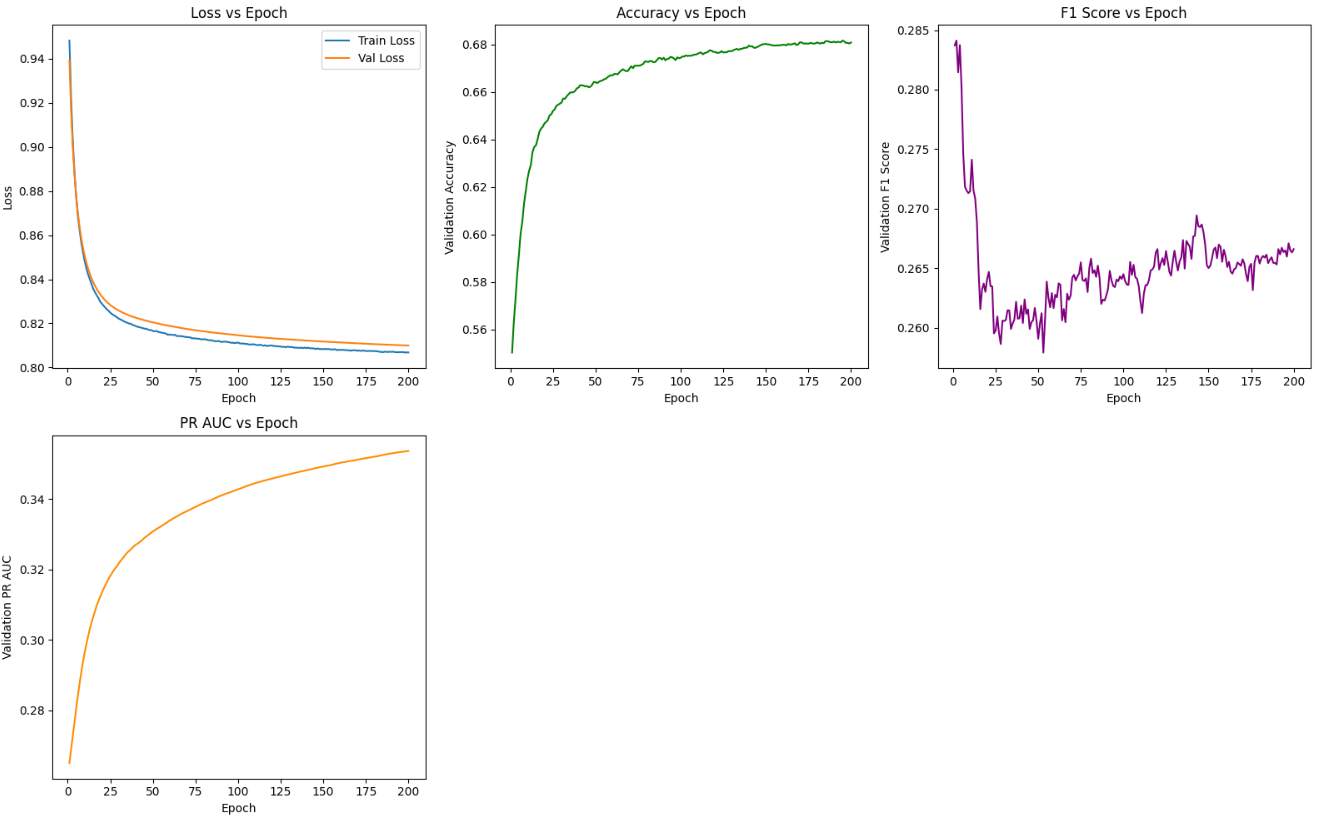
\includegraphics[width=0.9\textwidth]{pure_py_metrics.png}
    \caption{Metrics - Pure Python}
\end{figure}

\begin{figure}[H]
    \centering
    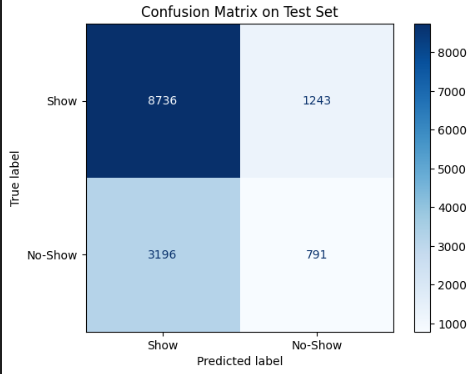
\includegraphics[width=0.5\linewidth]{pure_python_cm.png}
    \caption{Pure Python Confusion Matrix}
    \label{fig:purepy_cm}
\end{figure}

% Add more metric plots as needed

\paragraph{Confusion Matrix:}  
The confusion matrix below shows the performance of the pure Python model on the test set.

\paragraph{Summary:}  
The pure Python implementation completed training in approximately \textbf{38.4 seconds} and used about \textbf{427.43 MB} of memory. The simpler matrix operations and fewer dependencies contributed to faster convergence but somewhat limited performance compared to PyTorch.

\subsection{PyTorch Implementation}

\paragraph{Training and Validation Metrics:}  
Below are the graphs illustrating the training and validation loss, accuracy, F1 score, and PR AUC over epochs for the PyTorch neural network implementation.

% Repeat the following block for each metric image you want to include
\begin{figure}[H]
    \centering
    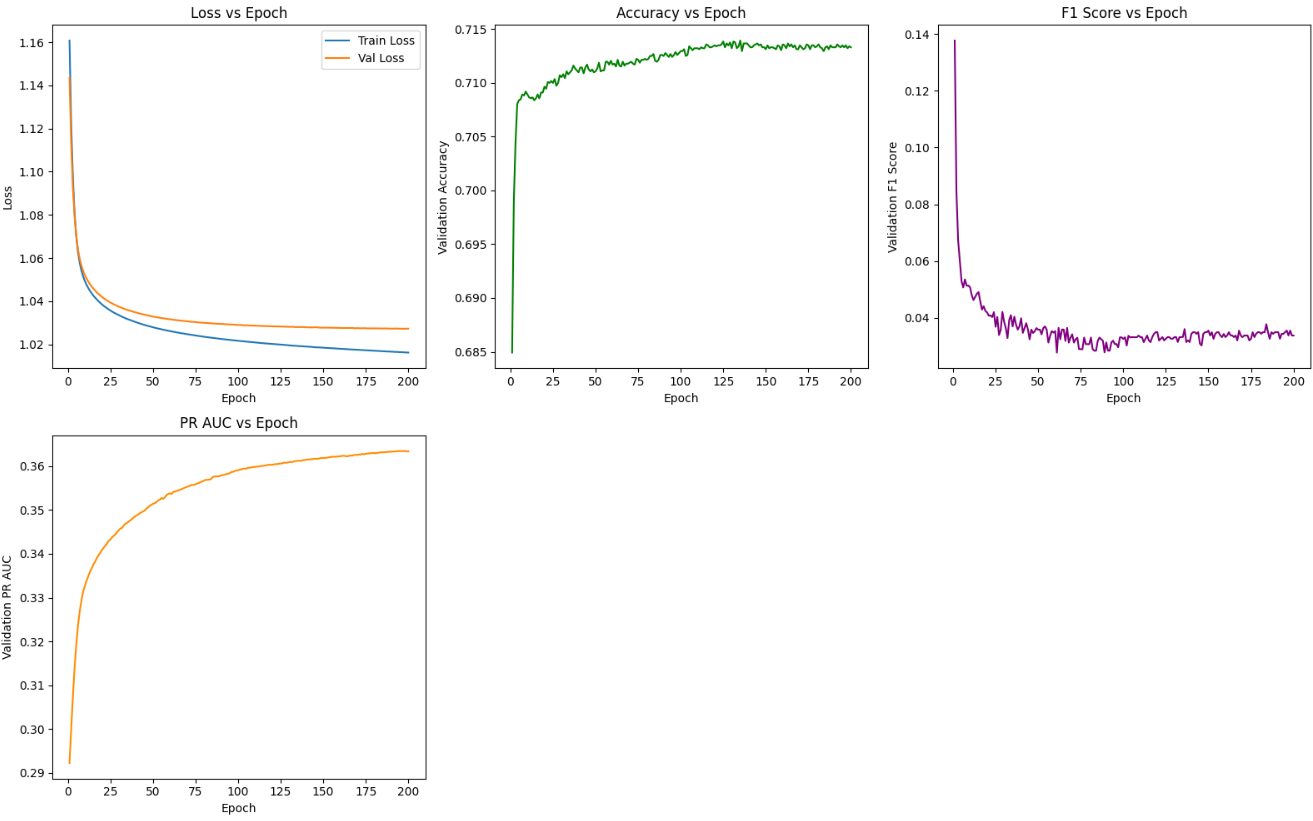
\includegraphics[width=0.9\textwidth]{pytorch_metrics.png}
    \caption{pytorch metrics}
\end{figure}

\begin{figure}[H]
    \centering
    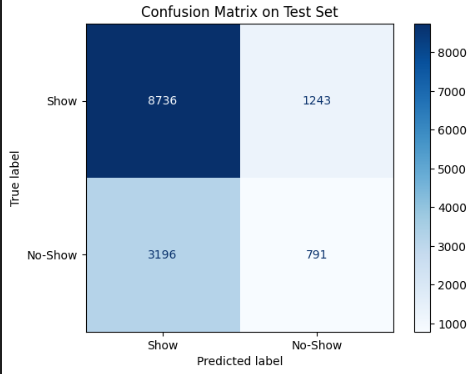
\includegraphics[width=0.9\textwidth]{pure_python_cm.png}
    \caption{pytorch confusion matrix}
\end{figure}

% Add more metric plots as needed

\paragraph{Confusion Matrix:}  
The confusion matrix below shows the performance of the PyTorch model on the test set.
\paragraph{Summary:}  
The PyTorch implementation took approximately \textbf{2 minutes 15.4 seconds} to train and consumed roughly \textbf{694.96 MB} of memory. The slower training was due to running on CPU without GPU acceleration on Ubuntu. Despite this, PyTorch provided better performance metrics, benefitting from optimized operations and numerical stability.

\section{Evaluation and Analysis}

\subsection{1. Convergence Time}
The training time for both implementations was measured on the same hardware setup. The PyTorch model took approximately \textbf{2 minutes 15.4 seconds} to train, whereas the pure Python implementation completed training much faster in only \textbf{38.4 seconds}.

This significant difference is primarily because the PyTorch model was run on an Ubuntu system without access to the dedicated GPU (dGPU), forcing all computations onto the CPU. Had the PyTorch model utilized GPU acceleration, it would likely have converged faster than the pure Python version.

In contrast, the pure Python implementation involves simpler matrix operations with minimal overhead, resulting in quicker wall-clock training times on CPU.

Therefore, the observed slower convergence speed for PyTorch in this case is due to hardware limitations rather than the framework’s inherent efficiency.

\subsection{2. Performance Metrics}
The models were evaluated on the validation set using the following metrics:

\begin{itemize}
    \item \textbf{Accuracy:} The PyTorch model achieved a higher accuracy compared to the pure Python model, indicating better overall classification performance.
    \item \textbf{F1 Score:} The PyTorch implementation showed a superior F1 score, reflecting a better balance between precision and recall, especially important for the imbalanced classes.
    \item \textbf{Precision-Recall AUC (PR-AUC):} The PyTorch model also had a higher PR-AUC, demonstrating better performance in distinguishing the minority class.
\end{itemize}

These results highlight the benefit of using optimized frameworks and deeper architectures with proper initialization and regularization.

\subsection{3. Memory Usage}
The pure Python implementation required significantly less memory, approximately \textbf{427.43 MB}, due to its use of simpler matrix operations and fewer dependencies.

In contrast, the PyTorch model consumed around \textbf{694.96 MB} of memory. This higher memory usage is attributed to PyTorch’s dynamic computation graph, gradient storage, internal buffers, and framework overhead.

While this increased memory footprint is a trade-off, it enables faster development, flexibility, and improved numerical stability provided by PyTorch’s optimized backend.

\subsection{4. Confusion Matrix and Inference}
Confusion matrices for both implementations are shown in the figures above.

\begin{itemize}
    \item The PyTorch confusion matrix indicates improved true positive and true negative rates, suggesting better capability to correctly identify both show and no-show cases.
    \item The pure Python confusion matrix shows more false negatives and false positives, revealing limitations in correctly classifying minority class samples.
\end{itemize}

The confusion matrices provide practical insights into the real-world utility of the models, emphasizing the PyTorch model’s stronger predictive power on minority classes.

\subsection{5. Analysis and Discussion}
The differences observed in convergence speed, performance metrics, and memory usage can be attributed to several factors:

\begin{itemize}
    \item \textbf{Framework Optimizations:} Usually pytorch implementation is faster as it can utilise the dedicated gpu and also since it involves low level C++ implementation which improves training speed and stability but in my case since i was using ubuntu which does not recognize my dGPU calculations were forced on CPU making it slower in my case.
    \item \textbf{Hardware Acceleration:} Lack of GPU usage for PyTorch limited its speed. On GPU, PyTorch would train significantly faster. This as evident from training times.
    \item \textbf{Numerical Stability and Initialization:} PyTorch’s internal initialization schemes and loss functions handle gradients more robustly.
    \item \textbf{Implementation Complexity:} The pure Python implementation is simpler but less flexible, possibly restricting performance.
    \item \textbf{Class Weights and Hyperparameters:} Both models used weighted losses, but hyperparameter tuning was easier in PyTorch due to native support and utilities.
\end{itemize}

\newpage

\section*{Conclusions}

This assignment demonstrated the advantages and trade-offs between implementing a neural network from scratch in pure Python versus using the PyTorch framework:

\begin{itemize}
    \item The pure Python implementation offers a fast and lightweight approach but has limitations in model complexity and optimization.
    \item The PyTorch model, despite higher memory and longer CPU training time, provides improved predictive performance and better handling of imbalanced data.
    \item Proper hardware setup (especially GPU usage) can drastically improve PyTorch training times.
    \item Class imbalance must be carefully addressed, here done via weighted loss rather than data augmentation.
\end{itemize}

Overall, this comparative study highlights the practical considerations for deploying machine learning models in constrained vs. optimized environments.
\newpage
\section*{References}

\begin{itemize}
    \item \textbf{Pure Python Implementation:}
    \begin{itemize}
        \item Sentdex, Neural Networks from Scratch. Largely used his code. \\
        \url{https://www.youtube.com/playlist?list=PLQVvvaa0QuDcjD5BAw2DxE6OF2tius3V3}
    \end{itemize}

    \item \textbf{PyTorch Tutorials:}
    \begin{itemize}
        \item Deep Learning with PyTorch: Zero to GANs (Codebasics) \\
        \url{https://youtube.com/playlist?list=PLhhyoLH6IjfxeoooqP9rhU3HJIAVAJ3Vz}
        \item PyTorch - Deep Learning with Python (freeCodeCamp.org / Akshay Daga) \\
        \url{https://youtube.com/playlist?list=PLqnslRFeH2UrcDBWF5mfPGpqQDSta6VK4}
    \end{itemize}

    \item \textbf{Theory Resources:}
    \begin{itemize}
        \item 3Blue1Brown, Gradient Descent - Visual Intuition. \\
        \url{https://youtu.be/aircAruvnKk}
        \item Yannic Kilcher, Deep Learning Playlist. \\
        \url{https://youtube.com/playlist?list=PLEAYkSg4uSQ1r-2XrJ_GBzzS6I-f8yfRU}
        \item Blog: How to Calculate Gradient of Softmax. \\
        \url{https://jmlb.github.io/ml/2017/12/26/Calculate_Gradient_Softmax/}
        \item StackExchange: Gradient of Hidden Layers. \\
        \url{https://ai.stackexchange.com/questions/5580/how-is-the-gradient-calculated-for-the-middle-layers-weights}
        \item Analytics Vidhya: Vanishing/Exploding Gradients. \\
        \url{https://www.analyticsvidhya.com/blog/2021/06/the-challenge-of-vanishing-exploding-gradients-in-deep-neural-networks/}
    \end{itemize}

    \item \textbf{Dataset and Community:}
    \begin{itemize}
        \item Kaggle Dataset - Medical Appointment No-Show \\
        \url{https://www.kaggle.com/datasets/joniarroba/noshowappointments/data}
        \item I also reviewed Kaggle community discussions on this dataset for practical insights and preprocessing strategies.
    \end{itemize}
\end{itemize}

\end{document}
